\documentclass[tikz,border=10pt]{standalone}
\usepackage{tkz-graph}
\usetikzlibrary{automata}
\usetikzlibrary[automata]
\begin{document}
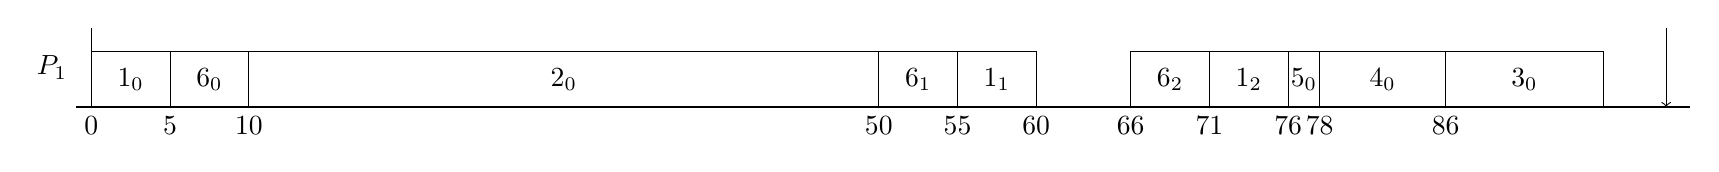
\begin{tikzpicture}
\draw (0,0) --(0,1) ;
\draw[<-] (20,0) ->(20,1) ;
\draw (-0.2,0) --(20.3,0) ;
\draw (0-0.5,0.5) node {$P_{1}$};
\draw (0,0) rectangle (1,0.7) node[pos=.5] {$1_0$};
\draw (0,0) node[below] {$0$};
\draw (1,0) rectangle (2,0.7) node[pos=.5] {$6_0$};
\draw (1,0) node[below] {$5$};
\draw (2,0) rectangle (10,0.7) node[pos=.5] {$2_0$};
\draw (2,0) node[below] {$10$};
\draw (10,0) rectangle (11,0.7) node[pos=.5] {$6_1$};
\draw (10,0) node[below] {$50$};
\draw (11,0) rectangle (12,0.7) node[pos=.5] {$1_1$};
\draw (11,0) node[below] {$55$};
\draw (12,0) node[below] {$60$};
\draw (13.2,0) rectangle (14.2,0.7) node[pos=.5] {$6_2$};
\draw (13.2,0) node[below] {$66$};
\draw (14.2,0) rectangle (15.2,0.7) node[pos=.5] {$1_2$};
\draw (14.2,0) node[below] {$71$};
\draw (15.2,0) rectangle (15.6,0.7) node[pos=.5] {$5_0$};
\draw (15.2,0) node[below] {$76$};
\draw (15.6,0) rectangle (17.2,0.7) node[pos=.5] {$4_0$};
\draw (15.6,0) node[below] {$78$};
\draw (17.2,0) rectangle (19.2,0.7) node[pos=.5] {$3_0$};
\draw (17.2,0) node[below] {$86$};
\end{tikzpicture}
\end{document}
